\section{Analisi preliminare}

Il sito web \textbf{html.it} è un periodico telematico specializzato nello sviluppo e nella programmazione web. Il sito è sviluppato da un team italiano e fornisce tutta una serie di \textbf{articoli} e \textbf{guide} su argomenti di varia natura. Si tratta di un sito web molto frequentato, personalmente ho attinto molto da questo sito web nei miei primi anni di programmazione. Attualmente lo visito poco spesso, in primo luogo perchè riguardo alla materia tendo a bazzicare altri siti e in secondo luogo perchè, come vedremo lungo questa relazione, giudico il suo grado di usabilità molto basso. Con questo non voglio certo screditare il suddetto, anzi, lo ritengo validissimo per contenuti e tematiche affrontate, ma d'altro canto ritengo che niente possa essere esentato da un giudizio critico costruttivo. In aggiunta tengo a precisare che molti aspetti della mia analisi sono liberamente opinabili e chiunque voglia biasimare alcune affermazioni o discutere è da me accolto benevolmente, purchè la discussione sia messa sul giusto piano.

\subsection{Struttura}

Il sito web, come detto, si occupa principalmente di mettere a disposizione guide utente semplici e basilari, in modo da incoraggiare l'utente ad approfondire o prendere contatto con un argomento. Ciascuna guida (o articolo) è normalmente \textbf{suddiviso in lezioni} che partono da concetti base fino ad approfondire gli aspetti più avanzati. Ciascuna guida è categorizzata secondo una struttura gerarchica. Possiamo vederla come un albero \textit{m}-ario in cui le foglie sono gli articoli o le guide e i nodi interni le categorie. Scendendo nell'albero la granularità si fa sempre più fine. Per capire il concetto possiamo riferirci alla figura seguente che raffigura un esempio:

\begin{figure}[htpd]
\centering
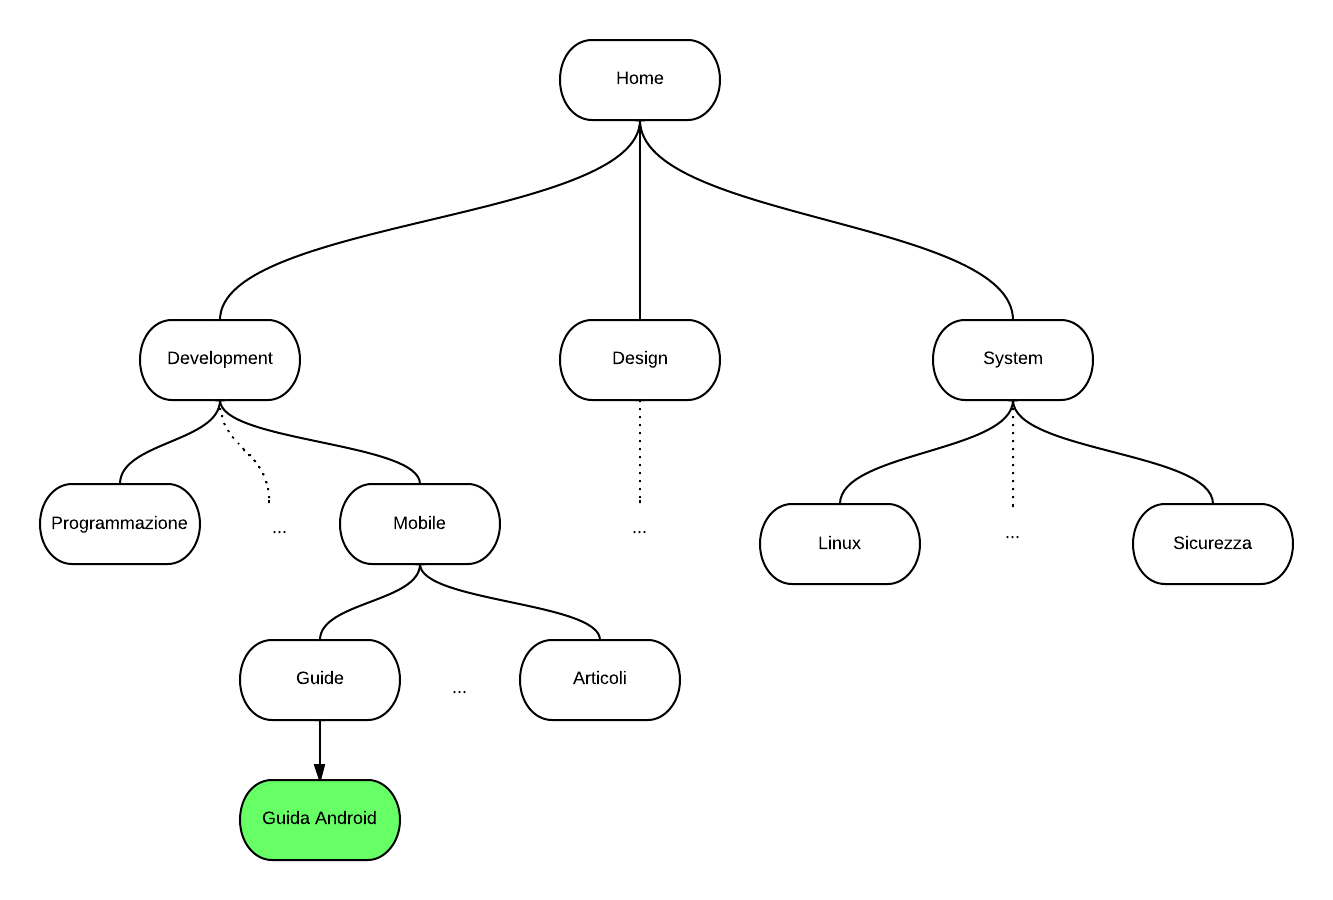
\includegraphics[width=120mm]{images/tree.png}
\caption{Struttura ad albero di html.it}
\end{figure}

In questo caso vediamo il formarsi di tre categorie principali:

\begin{itemize}

\item \textbf{Development}, contenente guide e articoli per lo sviluppo web, mobile, ecc;
\item \textbf{Design}, contiene guide e articoli per il design di applicazioni o siti web;
\item \textbf{System} che infine contiene guide e articoli per lo sviluppo e mantenimento di sistemi complessi, come ad esempio Linux.

\end{itemize}

Da queste tre categorie vi è una diramazione di sottocategorie con grana sempre più fine. Questa struttura consente all'utente di poter arrivare a ciò di cui necessita in tempi relativamente brevi.

\subsection{Sezioni}

Il sito è composto, oltre che delle sezioni riguardanti gli articoli e le guide, di altre sezioni ricche di contenuti:

\begin{itemize}

\item Una sezione \textbf{download}, dalla quale è possibile scaricare software o script generati dagli utenti;
\item Una sezione \textbf{video}, contenente una vera e propria libreria di video su un vastissimo numero di argomenti;
\item Una sezione \textbf{corsi}, in cui è possibile visualizzare una vetrina di corsi attinenti all'argomento;
\item Una sezione \textbf{forum} in cui gli utenti possono discutere di tutti gli argomenti attinenti al mondo dello sviluppo web (e non solo).

\end{itemize}

Analizzare tutte le sezioni risulterebbe un lavoro enorme e chiaramente più lungo del previsto, per cui ho deciso di analizzare solamente la sezione più navigata, ovvero quella relativa agli articoli e alle guide.